\section{Hierarchie výpočetní složitosti. P, P-úplné, NP, NP-úplné, PSPACE, EXP-SPACE, HP těžké, rozhodnutelné, nerozhodnutelné. Definice problému s~batohem. Definice problému k-řezu. Definice problému obchodu.}

\subsection{Polynomická vs exponenciální časová složitost.}

Algoritmy s~polynomickou složitostí lze efektivně řešit, bez vynaložení velkého výpočetního výkonu.
S~délkou vstupu \textit{n} roste lineárně potřebný čas ($n^x$) například hledání nejkratší cesty.
Algoritmy s~exponenciální složitostí lze efektivně řešit pouze pro~malé exponenty, bez potřeby velkého výpočetního výkonu.
S~délkou vstupu \textit{n} roste exponenciálně potřebný čas ($x^n$), například v~problému obchodního cestujícího.

\subsection{Hierarchie výpočetní složitosti.}

Hierarchie výpočetní složitosti slouží k~charakterizaci algoritmů u~kterých lze pouze nepřímo určit asymptotickou složitost.
Využívá se třídní hierarchie.
Třídy od nejjednodušší po nejsložitější jdou v~tomto pořadí: P $\subseteq$ P-úplné $\subseteq$ NP $\subseteq$ NP-úplné $\subseteq$ NP-těžké $\subseteq$ \#P $\subseteq$ PSPACE $\subseteq$ EXP $\subseteq$ HP-těžké $\subseteq$ neřešitelné.
Jednoduší třída je vždy podmnožinou složitější a~do~složitější patří i~ty jednoduší.

\subsubsection{Třída P}

Třída P obsahuje polynomiální problémy.
Tyto problémy se dají vyřešit v~polynomiálním čase na~deterministickém Turingově stroji (TS).
Příkladem může být nalezení nejkratší cesty, minimální kostry v~grafu.


\subsubsection{Třída P-úplné (P-complete)}
P-úplné problémy jsou nejtěžší problémy v~třídě P. Jsou to problémy, které jsou efektivně redukovatelné na všechny ostatní problémy v~třídě P. Pokud bychom našli polynomiální algoritmus pro jakýkoli P-úplný problém, bylo by možné efektivně řešit všechny problémy v~třídě P.

\subsubsection{Třída NP}

Třída NP obsahuje nedeterministické polynomiální problémy.
Tyto problémy lze řešit v~polynomiálním čase na~nedeterministickém TS (doposud nesestaven).

\subsubsection{Třída NP-complete (NP-úplné)}

NP-úplné (NP-Complete) je podskupina problémů třídy NP, která se zabývá rozhodovacími problémy.
Jejich řešení je nejtěžší a~všechna známá řešení lze na~deterministickém TS provést pouze s~exponenciálním čase.
Pro~polynomiální nebylo zatím nalezeno řešení, ale zároveň nebylo dokázáno, že řešení neexistuje.

\textbf{Problém NP-C}: pokud by se podařilo převést jeden NP-C problém na~polynomiální čas tak to znamená, že každý NP-C problém lze převést do~polynomiálního.
To by vedlo k~prokázání P $=$ NP.

Bylo dokázáno, že každý algoritmus pro~NP-C problém lze použít k~řešení jiného \mbox{NP-C} problému.
Přibližně existuje 10\,000 známých NP-C problémů.
Jde napříkald o~barvení grafů, Knapsnack (problém batohu), 3-partition problém (rozdělit množinu čísel na~podmnožiny o~velikosti 3 se stejným součtem), \dots

\subsubsection{Třída NP-těžké}

O~problému řekneme, že je NP-težký, jestliže se na~něj redukuje NP-C problém, ale zároveň nevíme jestli spadá do~NP.
Redukce znamená že se dá převést/konvertovat.

\subsubsection{P vs NP}

P~je podmnožina NP, jelikož každý problém lze řešit v~polynomiálním čase na
nedeterministickém TS.
Existuje matematický problém P $=$ NP, který dosud nebyl potvrzen nebo vyvrácen. Takže se přesně nedá určit jestli je P $=$ NP.
Obecně se považuje, že P $\neq$ NP.

\subsubsection{Třída \#P}

Třída \#P se nezabývá rozhodovacími problémy, ale řeší problém nalezení možných řešení NP problémů.
Z~toho plyne, že problémy třídy \#P musí být alespoň stejně složité jako stejný NP problém.
U~této třídy se neptáme jestli existuje řešení, ale kolik řešení existuje.

\textbf{Definice:} \#P je množina všech funkcí $f(x)$, kde $f(x)$ odpovídá počtu přijatelných cest nedeterministického TS v~polynomiálním čase.

V~této třídě existují také problémy \#P-úplné.

\subsubsection{Třída PSPACE}

PSPACE je množina rozhodovacích problémů, které lze vyřešit pomocí deterministického TS v~polynomiálním paměťovém prostoru.
Neboli nezáleží, jak dlouho trvá vykonání, když je využit polynomiální (rozumné) množství paměťi.
PSPACE má úplné problémy, které jsou sestupně samo redukovatelné (downward self-reducible) a~náhodně samo redukovatelné (random self-reducible).
Jsou zahrnuté v~EXP.
Dle Savitchova theorému můžeme dokázat, že \textbf{P}SPACE = \textbf{NP}SPACE.

\subsubsection{Třída EXP}

Často označována jako EXPTIME.
Je to množina rozhodovacích problémů řešitelných na~deterministickém TS v~exponenciálním čase.
Časová komplexita je O($2^{p(n)}$), kde $p(n)$ je polynomická funkce $n$.
Jejich složitost je exponenciální (například $2^n$).

Existuje také třída EXPSPACE, která je podobná EXPTIME, jen se neřeší v~exponenciálním času, ale v~exponenciálním paměťovém prostoru.

U~obou tříd se jedná o~nezvládnutelné problémy, pro~které neexistuje polynomiální algoritmus.

\subsubsection{Třída HP-těžké}
HP-těžké (Hard for the Polynomial hierarchy) problémy jsou alespoň tak obtížné jako nejtěžší problémy v~hierarchii P (Polynomial hierarchy).
Hierarchie P je hierarchie tříd složitosti P, NP, PSPACE, atd.
HP-těžké problémy jsou obtížné až na nejvyšší úrovni hierarchie P, která se skládá z~polynomiálního počtu vrstev.
Tyto problémy nelze efektivně řešit polynomiálním algoritmem na deterministickém Turingově stroji.
HP-těžké problémy jsou obecně obtížnější než NP-těžké problémy, protože jsou porovnávány s~vyšší úrovní hierarchie složitosti.
Třída HP-těžké je důležitá pro studium relací obtížnosti mezi různými třídami složitosti a~určování přesných hranic obtížnosti v~rámci hierarchie P.

\subsection{Rozhodnutelnost}

Rozhodnutelnost se týká schopnosti algoritmu správně rozhodnout, zda existuje efektivní metoda, kterou lze v~problému dojít ke správnému výsledku. Problém je rozhodnutelný, pokud existuje algoritmus, který pro každou instanci problému dá správnou odpověď "ano" nebo "ne". Rozhodnutelnost neříká nic o~efektivitě algoritmu nebo časové složitosti, zabývá se pouze jeho řešitelností.

\subsection{Problém batohu}

Zloděj má pro~krádeže připravený batoh s~určitou maximální hmotností/velikostí.
Při~krádeži se snaží do~batohu vložit co nejvíce zboží v~co největší hodnotě.
Každé toto zboží má jinou hmotnost/velikost a~jinou hodnotu.
Hledá nejlepší kombinaci zboží která se mu do~batohu vejde s~cílem maximalizovat profit.

\subsection{Problém k-řezu}

Problém k-řezu (anglicky "k-cut problem") je kombinatorický problém, který se zabývá rozdělením množiny uzlů v~grafu do dvou (nebo více) podmnožin tak, aby byl minimální počet hran, které překračují mezi těmito podmnožinami. Jinými slovy, cílem je najít řez grafu, který minimalizuje počet hran, které spojují uzly v~různých podmnožinách

\subsection{Problém obchodního cestujícího}

V~tomto NP-těžkém problému (\emph{Travelling Salesman Problem, TSP}) jde o~nalezení té nejkratší Hamiltonské cesty v~grafu $G$:
Hamiltonská cesta $P$ je taková cesta, která navštíví každý vrchol právě jednou.

Heurestické algoritmy negarantují že nalezly nejlepší řešení, ale operují v~dosažitelném čase.
Příkladem je \href{https://en.wikipedia.org/wiki/Nearest_neighbour_algorithm}{\emph{Nearest Neighbour}} (dochází k~\enquote{slepému} propojování nejbližších bodů bez~znalosti celku), který může vrátit nejlepší i~velmi špatný výsledek.

\subsubsection{Modifikace genetických algoritmů pro~TSP}

Genetické algoritmy nejdou na~TSP aplikovat přímo, protože každý z~vrcholů může být navštíven pouze jednou.

\begin{itemize}
    \item přirozený výběr: fitness funkce je celková délka cesty a~nevyžaduje modifikaci
    \item mutace: prohození dvou vrcholů uvnitř chromozomu nevyžaduje modifikaci
    \item křížení: nestačí vyměnit dvě části chromozomu, je třeba ho \enquote{přefiltrovat} a~vybrat pouze takové vrcholy, které se v~chormozomu ještě neobjevily (a~tyto vyfiltrované nahradit)
\end{itemize}

\subsection{Bonusové problémy}

\subsubsection{Problém směrování vozidel (VRP)}

Centrální sklad má $x$ vozidel.
Vozidla musí objet všechna zásobovací místa, dovést tam zboží a~vrátit se zpět.
Nemusí navštívit stejný počet míst, ale dohromady musí navštívit všechna místa co nejoptimálněji.
Pro~$x=1$ jde o~problém obdobný problému obchodního cestujícího, ale je zde navíc určen začátek cesty.

\subsubsection{Metrický k-střed}

$x$ měst má mezi sebou přesně definované vzdálenosti.
Mezi nimi (resp. do~nějakých z~měst) lze umístit $n$ skladišť která budou všechna města obsluhovat.
Cílem je vybrat nejvhodnější města pro~postavení skladu, aby maximální vzdálenost každého města ke~skladu byla co nejmenší.

\clearpage
\section{Optimalizace: Genetické programování, inicializace, křížení, mutace. Optimalizace rojem částic. Optimalizace mravenčí kolonií}

\subsection{Genetické programování}

Genetické programování pracuje se~stromy, ne vektory.
Strom obsahuje pouze funkce a~terminály (které jsou pouze v~listech a~nemají potomky).

Náhodně generované programy využívají základní operace a~konstanty pro~rozhodovací strom s~omezenou hloubkou.
Vybraná funkce rekurzivně generuje další stromy.

\subsubsection{Inicializace}

Inicializace je důležitým krokem v~genetických algoritmech, který se provádí na začátku evolučního procesu. Jeho účelem je vytvořit počáteční populaci jedinců, se kterými se bude pracovat v~algoritmu.
Existuje několik přístupů k~inicializaci populace v~genetických algoritmech. Některé z~běžných technik zahrnují:

\begin{description}
    \item[Náhodná] Jednoduchým způsobem inicializace je náhodné generování jedinců s~náhodnými genetickými hodnotami. Každý gen je inicializován náhodně z~rozmezí možných hodnot.
    \item[Heuristická] Při heuristické inicializaci se používají určité heuristiky nebo znalosti o~problému k~vytvoření počáteční populace. Tento přístup může vést k~lepšímu rozložení jedinců v~prostoru řešení a~snížit počet iterací potřebných k~dosažení optimálního řešení.
    \item[Inicializace z~předchozích znalostí] Pokud jsou dostupné předchozí znalosti o~problému, mohou být tyto informace využity k~inicializaci populace. Například pokud byla nalezena dobrá řešení v~minulosti, mohou být tyto řešení použity jako součást počáteční populace.
\end{description}

\subsubsection{Operace}

Stromy se kříží prohozením podstromů.

\begin{description}
    \item[Mutace] Mutace je náhodný proces, který způsobuje změnu jedince v~populaci. Cílem mutace je zachovat diverzitu a~předcházet přílišné konvergenci algoritmu k~lokálním optimům. Mutace provádí náhodné změny v~genetickém materiálu jedince, jako je změna jednoho nebo více genů, vkládání nebo vymazání genů nebo inverze genetických částí.
    \item[Křížení] Křížení je operátor, který kombinuje genetický materiál dvou nebo více jedinců a~vytváří nové potomky. Cílem křížení je kombinovat užitečné vlastnosti rodičů a~generovat potomky s~lepšími vlastnostmi. Existuje několik různých technik křížení, z~nichž nejčastější je jednobodové křížení, kde je genetický materiál vyměňován na jednom náhodně vybraném bodě. Dalšími technikami jsou například dvoubodové křížení, uniformní křížení nebo lineární křížení.
\end{description}

\begin{figure}[ht]
    \centering
    \tikzstyle{node}=[circle, draw, text centered]
    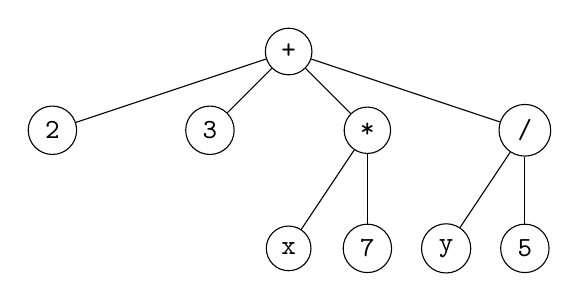
\begin{tikzpicture}
        \node[node](+) at (3, 3) {\texttt{+}};

        \node[node](2) at (0, 2) {\texttt{2}};
        \node[node](3) at (2, 2) {\texttt{3}};
        \node[node](*) at (4, 2) {\texttt{*}};
        \node[node](/) at (6, 2) {\texttt{/}};

        \node[node](x) at (3, 0.5) {\texttt{x}};
        \node[node](7) at (4, 0.5) {\texttt{7}};
        \node[node](y) at (5, 0.5) {\texttt{y}};
        \node[node](5) at (6, 0.5) {\texttt{5}};

        \begin{scope}[every path/.style={-}, every node/.style={inner sep=1pt}]
            \draw (2) -- node {} (+);
            \draw (3) -- node {} (+);
            \draw (*) -- node {} (+);
            \draw (/) -- node {} (+);

            \draw (x) -- node {} (*);
            \draw (7) -- node {} (*);
            \draw (y) -- node {} (/);
            \draw (5) -- node {} (/);
        \end{scope}
    \end{tikzpicture}
    \caption{Strom řešící příklad $5 + 7x + y/5 = 0$}
\end{figure}
\FloatBarrier

\subsection{Optimalizace rojem částic}

Optimalizace rojem částic (Particle Swarm Optimization, PSO) je metaheuristický algoritmus, který simuluje chování hejna částic při hledání nejlepšího řešení v~daném prostoru.
Algoritmus pracuje s~populací částic, které se pohybují ve vícedimenzionálním prostoru.
Každá částice má svou polohu a~rychlost, která určuje směr a~rychlost pohybu.
Částice se vzájemně ovlivňují a~sdílejí informace o~nejlepším nalezeném řešení v~prostoru.
Pohyb částic je řízen kombinací osobního nejlepšího řešení (lokální informace) a~nejlepšího řešení nalezeného v~celém hejnu (globální informace).
Algoritmus iterativně upravuje polohu a~rychlost částic, s~cílem najít co nejlepší řešení dané optimalizační úlohy. Je vhodný pro hledání globálních extrémů, například v~optimalizaci funkcí a~v~ladění parametrů modelů.

$$X(t+1) = X(t) + V(t+1)$$
$$V(t+1) = WV(t) + C_1 \cdot \mathrm{\texttt{rand()}} X (X_\mathrm{pbest} - X(t)) + C_2 \cdot \mathrm{\texttt{rand()}} X (X_\mathrm{gbest} - X(t))$$
%
kde $V(t)$ je rychlost v~čase $t$, $X(t)$ je pozice v~čase $t$, $W$ je váha, $C_1$/$C_2$ jsou učící a~akcelerační faktory, \texttt{rand()} je reálné číslo $\left<0, 1\right>$, $X_\mathrm{pbest}$ je nejlepší osobní pozice částice a~$X_\mathrm{gbest}$ je globální nejlepší pozice.

Jedna iterace algoritmu, tj. výpočet fitness funkce, probíhá ve~třech krocích:

\begin{enumerate}
    \item aktualizace osobního i~globálního nejlepšího výsledku,
    \item aktualizace rychlosti částic,
    \item aktualizace pozice částic.
\end{enumerate}

\subsection{Optimalizace mravenční kolonií}

Mravenčí kolonie (ACO) je metaheuristický algoritmus, který simuluje chování mravenců při hledání nejlepších tras v~prostoru.
Algoritmus se inspiruje komunikací a~kooperací mravenců při hledání potravy a~vytváření feromonových stop.
Mravenci se pohybují po grafu reprezentujícím problémovou instanci.
Každý mravenec si pamatuje svou cestu a~zanechává feromony na navštívených hranách.
Feromony slouží jako pozitivní zpětná vazba, která mravence láká k~vybrání stejné cesty jako ostatní mravenci.
Mravenci většinou preferují cesty s~vyšší koncentrací feromonů, ale zároveň dochází k~postupnému vyprchávání feromonů.
Algoritmus iterativně aktualizuje koncentrace feromonů a~vylepšuje kvalitu nalezeného řešení. Je vhodný pro hledání nejkratších cest v~grafech a~optimalizaci v~oblastech jako plánování tras, rozvrhování a~telekomunikace.

Simuluje mnoho nezávislých kooperujících jedinců:

\begin{enumerate}
    \item vytvoření částečného řešení,
    \item přidání hrany na~základě stochastických parametrů a~feromonů,
    \item vyhledání lokálního minima,
    \item aktualizace feromonů dobrých řešení.
\end{enumerate}

% \subsection{Evoluční strategie}
% 
% Využívá pouze mutaci, ne křížení.
% Jednotlivci jsou většinou reprezentováni jako pár vektorů reálných čísel: $v = (x, \sigma)$, kde $x$ je souřadnice pozice a~$\sigma$ je vektor směrodatných odchylek v~daném bodu.

\clearpage
\section{Grafy -- incidenční matice, matice sousedností. Handshaking lemma. Silně propojené komponenty grafu -- Kosarajův algoritmus, Tarjanův algoritmus}

Graf je matematická struktura $G = (V, E)$: uspořádaná dvojice množin vrcholů a~hran (\emph{vertices and edges}), kde hrana je určena dvěma vrcholy a~volitelně směrem nebo váhou.
Velké množství problémů postavených nad~grafy je NP-úplných.

\subsection{Maticové reprezentace}

\begin{description}
    \item[Incidenční matice] obsahuje informace o~mapování vrcholů jednotlivým hranám.
        Matice má řádek pro~každý vrchol a~sloupec pro každou hranu; pokud vrchol hraně náleží, je na~pozici jednička (pro~orientované grafy může mít výchozí vrchol hodnotu $-1$).
    \item[Matice souslednosti] má podobu čtvercové matice $n \times n$ (kde $n$ je počet vrcholů grafu), jejíž hodnota na~místě $a_{i,j}$ je celé číslo odpovídající počtu hran vedoucích z~vrcholu $i$ do~vrcholu $j$, prvky na~diagonále pak odpovídají počtu hran vedoucích z~vrcholu $i$ do~vrcholu $i$.
\end{description}


\begin{figure}[ht!]
    \centering
    \begin{minipage}{0.25\textwidth}
        \centering
        \includegraphics[height=8em]{images/3_graf-matice-souslednosti}
        \caption[Ilustrační graf]{Ilustrační graf}
        \label{ilustracni-graf-matice}
        {\tiny (Chris-martin, Wikimedia Commons, volné dílo)}
    \end{minipage}%
    %
    \begin{minipage}{0.35\textwidth}
        \centering
        $\left( \begin{matrix}
                    2 & 1 & 1 & 0 & 0 & 0 & 0 \\
                    0 & 1 & 0 & 1 & 0 & 0 & 0 \\
                    0 & 0 & 0 & 1 & 1 & 0 & 0 \\
                    0 & 0 & 0 & 0 & 1 & 1 & 1 \\
                    0 & 0 & 1 & 0 & 0 & 1 & 0 \\
                    0 & 0 & 0 & 0 & 0 & 0 & 1 \\
                \end{matrix} \right)$
        \caption[Incidenční matice]{Incidenční matice}
        (vrcholy a~hrany)
        % https://sciencedirect.com/topics/mathematics/incidence-matrix
    \end{minipage}%
    %
    \begin{minipage}{0.3\textwidth}
        \centering
        $\left( \begin{matrix}
                    2 & 1 & 0 & 0 & 1 & 0 \\
                    1 & 0 & 1 & 0 & 1 & 0 \\
                    0 & 1 & 0 & 1 & 0 & 0 \\
                    0 & 0 & 1 & 0 & 1 & 1 \\
                    1 & 1 & 0 & 1 & 0 & 0 \\
                    0 & 0 & 0 & 1 & 0 & 0 \\
                \end{matrix} \right)$
        \caption[Matice souslednosti]{Matice souslednosti}
        (vrcholy k~vrcholům: diagonálně symetrická)
    \end{minipage}
\end{figure}
\FloatBarrier

\subsection{Handshaking lemma}

Handshaking lemmma je tvrzení že pro~každý konečný neorientovaný graf platí, že počet vrcholů s~lichým stupněm je sudý (formálně $\sum_{v \in V} \deg v = 2 |E|$: součet stupňů vrcholů odpovídá dvojnásobku počtu hran).

V~roce 1736 byla dokázána Leonardem Eulerem v~dokumentu řešícím problém Sedmi mostů města Královce\footnote{\url{https://en.wikipedia.org/wiki/Seven_Bridges_of_Konigsberg}}.
Graf obsahuje Eulerovskou cestu právě tehdy, když jím lze projít tak, aby byla každá hrana navštívena právě jednou.

\subsection{Silně propojené komponenty}

\emph{Graf} je silně propojený tehdy, když je každý vrchol dosažitelný z~každého jiného vrcholu.
Silně propojené komponenty jsou podgrafy, které jsou samy o~sobě pevně propojeny.

\subsubsection{Kosarajův algoritmus}

Kosarajův algoritmus je algoritmus pro nalezení silně propojených komponent v~orientovaném grafu pracující v~lineárním čase.. Jeho základní myšlenkou je provést dva průchody grafem - první průchod pro získání "finishing times" (čas dokončení) uzlů a~druhý průchod pro nalezení silně propojených komponent.
% TODO Tato poznámka je sice pravdivá, ale není zřejmá z pseudokódu
% Využívá faktu, že transponovaný graf $G^T$ má stejné silně propojené komponenty jako původní graf $G$.

% TODO ^^ Blbě! https://www.youtube.com/watch?v=Jb1XlDsr46o

\subsubsection{Tarjanův algoritmus}

Další efektivní algoritmus pro nalezení silně propojených komponent v~orientovaném grafu, efektivnější než Kosarajův. Jeho základní myšlenkou je použít hloubkové prohledávání (DFS) spolu s~nízkými čísly (lowlink) uzlů pro identifikaci silně propojených komponent. Neobrací orientace hran, pokud se do nějakého vrcholu vrátím -- nastavím mu výstupní hodnotu jako hodnotu předka vrcholu, do kterého vstoupil, pracuje se zásobníkem

\begin{figure}[htbp]
    \begin{minipage}{0.45\textwidth}
        \small
        \onehalfspacing
        \begin{enumerate}
            \item Označ každý vrchol grafu za~nenavštívený
            \item Vytvoř zásobník $L$
            \item Pro každý vrchol grafu $u$ spusť podprogram Navštiv($u$):
                  \begin{itemize}
                      \item Pokud je $u$ nenavštívený:
                            \begin{enumerate}
                                \item Označ $u$ jako navštívený
                                \item Pro každého souseda $n$ zavolej Navštiv($n$)
                                \item Přidej $u$ na~vrchol zásobníku
                            \end{enumerate}
                      \item Jinak nedělej nic
                  \end{itemize}
            \item Pro každý vrchol $u$ zásobníku $L$ spusť podprogram Přiřaď($u$, $u$):
                  \begin{itemize}
                      \item Pokud $u$ nepatří žádné komponentě:
                            \begin{enumerate}
                                \item Přiřaď $u$ komponentě $A$
                                \item Pro každého souseda $n$ zavolej Přiřaď($n$, $u$)
                            \end{enumerate}
                      \item Jinak nedělej nic
                  \end{itemize}
        \end{enumerate}
        \caption{Kosarajův algoritmus}
        \label{fig:kosaraj}
    \end{minipage}
    \hfill
    \begin{minipage}{0.45\textwidth}
        \small
        \onehalfspacing
        \begin{enumerate}
            \item Označ každý vrchol grafu za~nenavštívený
            \item Vytvoř zásobník
            \item Vytvoř čítač \emph{i} a~nastav ho na~1
            \item Vyber nenavštívený vrchol \emph{v} a~spusť nad ním podprogram Propoj(\emph{v}):
                  \begin{enumerate}
                      \item nastav \emph{v.index} a~\emph{v.lowlink} na~\emph{i}
                      \item zvyš čítač \emph{i} o~1
                      \item přidej vrchol \emph{v} do~zásobníku
                      \item pro každého navštívitelného souseda \emph{n}:
                            \begin{itemize}
                                \item pokud \emph{n} nebyl navštíven, nastav \emph{v.lowlink} na~\emph{min(v.lowlink, n.lowlink)}
                                \item pokud je \emph{n} v~zásobníku, nastav \emph{v.lowlink} na~\emph{min(v.lowlink, n.index)}
                            \end{itemize}
                      \item pokud je \emph{v.lowlink} rovný \emph{v.index}:
                            \begin{enumerate}
                                \item vytvoř propojenou komponentu ze zásobníku
                                \item vymaž zásobník
                            \end{enumerate}
                  \end{enumerate}
        \end{enumerate}
        \caption{Tarjanův algoritmus}
        \label{fig:tarjan}
    \end{minipage}
\end{figure}
\FloatBarrier

\begin{figure}[ht]
    \centering
    \includegraphics[width=\textwidth]{images/3_tarjanuv-algoritmus-animace.png}

    \caption[Animace Tarjanova algoritmu]{Animace Tarjanova algoritmu\\{\small (LynX, Wikimedia Commons, CC BY-SA 3.0)}}
\end{figure}

\clearpage
\section{Detekce cyklů v~grafu. Eulerova cesta grafem, Hamiltonovská cesta grafem. Floyd-Warhsallův algoritmus. Algoritmus rozpoznání bipartitiního grafu.}

\subsection{Detekce cyklů v~grafu}

Detekce cyklů v~grafech je důležitý problém v~teorii grafů s~mnoha praktickými aplikacemi:

\begin{itemize}
    \item Zajišťuje správnost algoritmů, které pracují s~grafy.
    \item Pomáhá odhalovat závislosti a~cyklické struktury v~aplikacích jako je plánování projektů nebo analýza sociálních sítí.
    \item Hraje roli při optimalizaci obchodních procesů a~řízení toku materiálu.
    \item Poskytuje cenné informace pro řešení problémů a~zlepšení výkonnosti systémů a~procesů.
\end{itemize}

\subsection{Eulerova cesta grafem}

Eulerova cesta je cesta v~grafu, která projde každou hranou právě jednou. Eulerův cyklus je Eulerova cesta, která začíná a~končí ve stejném vrcholu. Graf, který obsahuje Eulerův cyklus, se nazývá Eulerův graf. Patří do P.

\subsection{Hamiltonovská cesta grafem}

Hamiltonovská cesta je cesta v~grafu, která projde každým vrcholem právě jednou. Hamiltonovský cyklus je Hamiltonovská cesta, která začíná a~končí ve stejném vrcholu. Graf, který obsahuje Hamiltonovský cyklus, se nazývá Hamiltonovský graf. Patří do NP-complete.

\subsection{Floyd-Warshallův algoritmus}

Floyd-Warshallův algoritmus je algoritmus pro nalezení nejkratších cest mezi všemi dvojicemi vrcholů v~ohodnoceném orientovaném nebo neorientovaném grafu. Algoritmus používá dynamické programování a~postupně aktualizuje matice vzdáleností mezi vrcholy.


\subsection{Detekce bipartitního grafu}

Graf je bipartitní\footnotemark[1], pokud lze jeho vrcholy rozdělit na dvě skupiny tak, že žádné dvě vrcholy ve stejné skupině nejsou spojeny hranou.

\footnotetext[1]{Bipartitní graf G je definován jako dvojice $(V, E)$, kde $V$ je množina vrcholů a~$E$ je množina hran. Je-li $V$ rozdělena na dvě disjunktní množiny $V_1$ a~$V_2$ ($V = V_1 \cup V_2$, $V_1 \cap V_2 = \emptyset$), pak každá hrana v~$E$ spojuje vrchol z~množiny $V_1$ s~vrcholem z~množiny $V_2$.}

\begin{figure}[htbp]
    \begin{minipage}{0.55\textwidth}
        \small
        \onehalfspacing
        \begin{enumerate}
            \item Vyber bod grafu.
            \item Přiřaď mu barvu a~označ ho za~navštívený.
            \item Procházej vrcholy grafu a~postupně je přiřazujte jednu z~dvou barev (A~nebo B), pokud ještě nejsou přiřazeny tak, aby sousední vrcholy neměly stejnou barvu.
            \item Pokud narazíš na hranu, která spojuje dva vrcholy stejné barvy, graf není bipartitní.
            \item Pokračuj, dokud nejsou všechny vrcholy přiřazeny barvou.
        \end{enumerate}
        \caption{Rozpoznání bipartitního grafu}
        \label{fig:alg-barveni}
    \end{minipage}
    \hfill
    \begin{minipage}{0.35\textwidth}
        \small
        \onehalfspacing
        \centering
        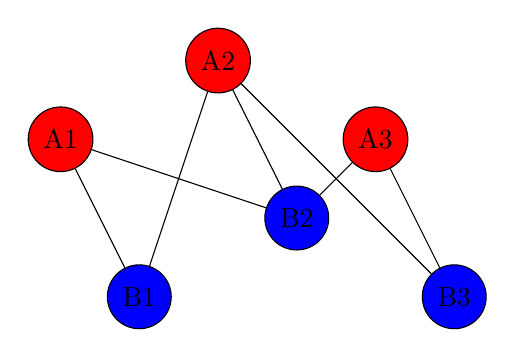
\begin{tikzpicture}
            % Definice vrcholů
            \node[draw, circle, fill=red] (A1) at (0,0) {A1};
            \node[draw, circle, fill=red] (A2) at (2,1) {A2};
            \node[draw, circle, fill=red] (A3) at (4,0) {A3};
            \node[draw, circle, fill=blue] (B1) at (1,-2) {B1};
            \node[draw, circle, fill=blue] (B2) at (3,-1) {B2};
            \node[draw, circle, fill=blue] (B3) at (5,-2) {B3};

            % Hrany mezi vrcholy
            \draw (A1) -- (B1);
            \draw (A1) -- (B2);
            \draw (A2) -- (B1);
            \draw (A2) -- (B2);
            \draw (A2) -- (B3);
            \draw (A3) -- (B2);
            \draw (A3) -- (B3);
        \end{tikzpicture}
        \caption{Bipartitní graf}
        \label{fig:bipartitni-graf}
    \end{minipage}
\end{figure}
\FloatBarrier

\clearpage
\section{Párování grafu, problém maximální shody -- definice, Maďarský algoritmus. Problém časové tabule. Algoritmus barvení grafu. Isomorfismus grafu -- Ullmanův algoritmus.}

% Excentricita vrcholu $x$ grafu $G$ je maximální vzdálenost bodu od~jakéhokoliv bodu v~grafu: $\mathrm{e}(x) = \max\{ d_G(x, y) \ |\ y \in V_G\}$, kde $d_G(x,y)$ je minimální vzdálenost mezi body $x, y$.
% 
% {}Pro~poloměr grafu platí $\mathrm{r}(G) = \min\{ \mathrm{e}(x)\ |\ x \in V \}$.
% \\Pro~průměr grafu platí $\mathrm{d}(G) = \max\{ \mathrm{e}(x)\ |\ x \in V \}$.

\subsection{Párování grafu}

Párování grafu se týká propojení hranami vrcholů v~grafu. V~neorientovaném grafu je párování množina hran, které spojují vrcholy tak, aby se žádné dva vrcholy nesdílely stejnou hranu. Maximální shoda je párování s~co největším počtem hran. V~orientovaném grafu je párování množina hran, které vycházejí z~vrcholů a~vedou k~jiným vrcholům, přičemž každý vrchol je spojen maximálně s~jednou hranou. Párování grafu se používá v~různých aplikacích, jako je plánování úkolů, rozvrhování a~mapování v~překladačích.

% Párování grafu je taková podmnožina hran grafu $M \subseteq E$, ve~které žádné dvě hrany nemají společný vrchol.
% Vrcholy, které patří do~párování, se nazývají \emph{saturované}.
% 
% {}\emph{Maximální} párování má nejvíce hran (protože graf může mít párování více).
% \\\emph{Perfektní} párování pokrývá všechny vrcholy grafu.

\subsection{Problém maximální shody}

Problém maximální shody se týká hledání největší možné množiny hran v~grafu, kde žádné dvě hrany nesdílejí společný vrchol. Cílem je najít co největší počet hran, které se nepřekrývají. Tento problém má různé aplikace, například při hledání nejlepšího párování mezi lidmi v~sociální síti. Existuje několik algoritmů pro řešení tohoto problému, které postupně rozšiřují párování a~hledají nejlepší kombinace hran.

\subsubsection{Maďarský algoritmus}

Vstupem je matice $m \times n$ (řádky odpovídají \enquote{pracovníkům} a~sloupce \enquote{úkolům}).

\begin{enumerate}
    \item Všem polím v~každém řádku odečti nejnižší hodnotu řádku.
    \item Všem polím v~každém sloupci odečti nejnižší hodnotu sloupce.
    \item Nakresli čáru přes řádky/sloupce tak aby byly překryty všechny nuly co nejmenším počtem čar (= pokrytí).
    \item Pokud je počet čar roven počtu řádků, algoritmus končí.
    \item Najdi nejmenší nepokrytou hodnotu. Odeči její hodnotu od~každého odkrytého řádku a~přidej ji ke~každé nenulové hodnotě v~zakrytému sloupci. Vrať se na~krok~3.
\end{enumerate}

Výsledkem je nějaká možnost z~existujících kombinací nenulových polí.

\subsection{Problém časového rozvrhu}

Ve~škole je $m$ učitelů a~$n$ tříd.
Učitel $i$ musí učit v~třídě $j$ v~semestru $P_{i,j}$.
Problémem je nalezení nejlepšího řešení.

Existuje mnoho verzí tohoto problému:
limitovaný počet učeben,
učitelé mohou učit jen v~určité časy,
žáci musí mít obědovou pauzu,
v~rozvrhu by neměly být zbytečné díry,
\dots

\subsubsection{Barvení grafů}

Barvení grafu je úloha přiřazení barev vrcholům grafu tak, aby žádné dva sousedící vrcholy neměly stejnou barvu. Cílem je použít co nejméně barev k~obarvení grafu, přičemž dodržujeme pravidlo není si sousedících vrcholů.

Problém barvení grafu má významné aplikace v~oblastech jako plánování rozvrhu, mapování registru v~překladačích, plánování v~bezdrátových sítích a~dalších oblastech, kde je potřeba přiřadit omezené zdroje různým prvky grafu tak, aby nedocházelo ke konfliktům.

\paragraph{Largest Degree Ordering}

Vrcholy grafu jsou seřazeny sestupně dle jejich stupně.
Prochází se jimi postupně: vrchol je obarven takovou nejdřívější barvou, která se nevyskytuje u~jeho sousedů.

\paragraph{Incidence Degree Ordering}

Je vybrán vrchol s~nejvyšším stupněm, kterému je přiřazena první barva.
Pro~neobarvené vrcholy je spočítán počet obarvených sousedů a~k~obarvení je vybrán ten s~jejich největším počtem.

\subsection{Izomorfismus grafů}

Izomorfismus\footnote{Mějme dva grafy $G = (V, E)$ a~$H = (U, F)$. Izomorfismus grafů $G$ a~$H$ je bijekce (odpovídající zobrazení) mezi množinami vrcholů $V$ a~$U$, která zachovává sousednost hran.
} grafů se zabývá porovnáváním dvou grafů a~zjišťováním, zda mají stejnou strukturu. Pokud jsou grafy izomorfní, znamená to, že jsou si podobné, i~když se mohou lišit v~označeních prvků. Cílem je najít takové přiřazení vrcholů mezi grafy, které zachovává jejich propojení. Existuje několik algoritmů pro testování izomorfismu grafů, ale pro složitější grafy je obtížné nalézt obecně efektivní řešení. Izomorfismus grafů je důležitý, protože nám umožňuje porovnávat grafy a~analyzovat jejich strukturu.


% TODO Způsoby rozpoznání

\subsubsection{Ullmanův algoritmus}
\begin{itemize}
    \item algoritmus pro určení, zda graf G má subgraf G', který by byl isomorfní ke grafu P
    \item pro představu: máme obrázek na krabici s~puzzle (G) a~chceme vědět, kam konkrétní dílek puzzle (P) zapadá, pokud vůbec
    \item NP-complete problém, protože speciální případ je Hamiltonovský cyklus
\end{itemize}

\clearpage
\section{Definice toku sítí. Problém maximálního toku/minimálního řezu. Ford--Fulkersonův algoritmus.}

Tok v~síti je koncept v~teorii grafů, který popisuje proudění zdrojů (např. voda, energie, data) mezi uzly sítě přes hrany. Síť se skládá z~orientovaných hran a~vrcholů, přičemž každá hrana má svou kapacitu, což je maximální množství toku, které může přenést.

\subsection{Maximální tok grafem}

Maximální tok a~minimální řez jsou dva výrazy popisující stejný problém, pouze na~něj nahlíží z~jiných stran.

Pracuje se s~orientovaným váženým grafem $G$ se zdrojem $s$ a~cílem $t$, kde pro~každou hranu $e$ platí $c(e) \geq 0$ (kde $c$ je kapacita hrany).

Celkový tok na~vstupu se musí rovnat toku na~výstupu, každý nezdrojový a~neterminální bod musí mít shodnou kapacitu na~vstupu a~výstupu.

Pokud je vstupních/terminálních bodů více, nejsnažší řešení je jejich sloučení do~virtuálního uzlu s~nekonečnou kapacitou.

\subsubsection{Ford--Fulkersonova metoda}

Ford-Fulkersonův algoritmus je jedním z~algoritmů používaných k~řešení problému maximálního toku v~síti. Algoritmus postupně hledá zlepšující cesty mezi zdrojem a~cílem, což jsou cesty, které umožňují zvýšit celkový tok v~síti. V~každém kroku algoritmus najde zlepšující cestu pomocí například prohledávání do hloubky nebo šířky a~zvětší tok podél této cesty. Algoritmus pokračuje, dokud existuje zlepšující cesta, a~výsledkem je maximální tok v~síti.

Ford-Fulkersonův algoritmus je základním algoritmem pro řešení problému maximálního toku, ale existuje několik modifikací a~optimalizací tohoto algoritmu, jako je Edmonds-Karpův algoritmus, který využívá prohledávání do šířky. Algoritmus je efektivní pro řešení problému maximálního toku v~malých a~středně velkých sítích, ale pro velké sítě může být pomalý a~je třeba použít pokročilejší metody.

\begin{figure}[ht]
    \onehalfspacing
    \begin{enumerate}
        \item Začni s~nulovým tokem
        \item Dokud existují rozšiřující cesty:
              \begin{enumerate}
                  \item Najdi rozšiřující cestu pomocí BFS
                  \item Vypočítej úzké hrdlo pro danou cestu
                  \item Pro~každý vrchol $u \rightarrow v$ na cestě
                        \begin{enumerate}
                            \item Zvyš tok $u \rightarrow v$ o~hodnotu hrdla
                            \item Sniž tok $v \rightarrow u$ o~hodnotu hrdla
                        \end{enumerate}
                  \item Zvyš maximální tok o~hodnotu hrdla
              \end{enumerate}
    \end{enumerate}
\end{figure}

FFM není plně specifikována; když se hovoří o~algoritmu, nazývá se Edmonds--Karpovým algoritmem.

\begin{figure}[ht]
    \centering
    \includegraphics[height=25em]{images/5_edmonds-karp}
    \caption{Řešení maximálního proudu Edmonds--Karpovým algoritmem}
    {\small (Cburnett, Wikimedia Commons, CC BY-SA 3.0)}
    % TODO Cesta z D->E má být E->D
\end{figure}
\FloatBarrier

\subsection{Úzké hrdlo}

Úzké hrdlo cesty je minimální hodnota kapacity hrany na~této cestě.

Úzké hrdlo mezi dvěma vrcholy je maximum z~úzkých hrdel přes všechny cesty mezi těmito vrcholy.

Úzké hrdlo grafu je minimum z~úzkých hrdel cest mezi vstupem a~terminálem.

\subsection{Reziduální cesta}


Reziduální cesta (anglicky "residual path") je cesta v~síti toku, která má ještě volnou kapacitu pro zvýšení toku přes hrany. Je to cesta, kterou lze využít pro další zvýšení toku v~rámci Ford-Fulkersonova algoritmu pro hledání maximálního toku v~síti. Jedná se o~rozdíl kapacity a~proudu: $c_\mathrm{res}(u,v) = c(u,v) - f(u,v)$.

Reziduální cesta je cesta od~terminálu ke~vstupu vytvořená reziduálními hranami.

\clearpage
\section{Univerzální aproximační teorém. Neuron, Maticová verze dopředné neuronové sítě. Rychlost učení. Dávky a~minidávky a~efekt na~učení se. Vrstva zahazování.}

Univerzální aproximační teorém je matematické tvrzení, které říká, že dopředná neuronová síť s~dostatečně velkým počtem neuronů je schopna aproximovat libovolnou spojitou funkci na omezeném intervalu s~libovolnou přesností. Tento teorém poskytuje teoretický základ pro použití neuronových sítí jako univerzálních aproximátorů funkcí.
Neříká však nic o~způsobu konstrukce aktivační funkce.

\subsection{Neuron}

Neuron je základní stavební prvek neuronových sítí. Jedná se o~matematický model, který simuluje chování biologických neuronů. Neuron přijímá vstupní signály, provádí na nich váhovou sumaci a~předává výstupní signál pomocí aktivační funkce. V~neuronových sítích se neurony organizují do vrstev a~vzájemně propojují pomocí vah.

\subsection{Dopředná neuronová síť}

Jde o~nejstarší a~nejjednodušší typ sítí.
FFNN je umělá neuronová síť ve~které neurony netvoří cykly (čímž se liší od~rekurentních neuronových sítí).
Informace prochází od~vstupu přes (volitelné) skryté vrstvy do~vstvy výstupní.

Jednovrstvá síť (ve~které je vstup přímo napojen na~výstup) se nazývá \emph{perceptron}.
Vstupy jsou sečteny na~základě vah a~tvoří výslednou hodnotu (typicky jedinou).
Vzhledem ke~své limitaci se dokáže naučit pouze lineárně separovatelné funkce (mezi které \emph{ne}patří například XOR).
Reálně využívané FFNN však mají skrytých vrstev více.

Vícevrstvé sítě využívají různé způsoby učení a~nejpopulárnější z~nich je zpětná propagace (\emph{back-propagation}).
Výstupní hodnoty jsou porovnány se správnou odpovědí a~informace je různými způsoby vracena zpátky do~sítě.
Algoritmus takto mění váhy jednotlivých propojení mezi neurony tak aby se celková chyba o~trochu snížila.

Když je tento proces opakován v~dostatečně velkém počtu cyklů, síť konverguje a~její chybovost se přestane měnit.
Tento proces se nazývá gradientní sestup.

V~síti také může dojít k~přetrénování: FFNN se \enquote{moc zaměří} na~trénovací sadu a~přestane zachycovat opravdové statické vlastnosti datasetu.

\subsection{Maticová reprezentace NN}

Maticová verze dopředné neuronové sítě je způsob reprezentace vstupů, vah a~výstupů neuronové sítě pomocí matic. V~této reprezentaci jsou vstupy, váhy a~výstupy neuronů uspořádány do matic a~operace nad nimi jsou prováděny maticovým násobením. Maticová reprezentace usnadňuje výpočty a~urychluje zpracování dat v~neuronové síti.

\begin{figure}[ht]
    \onehalfspacing
    \centering
    \includegraphics[height=10em]{images/6_maticova-operace}
    $$
        \sigma \left(
        \underbrace{
            \left[ \begin{matrix}
                1  & -2 \\
                -1 & 1  \\
            \end{matrix} \right]
        }_{\mathrm{v\acute{a}hy}}
        \underbrace{
            \left[ \begin{matrix}
                1  \\
                -1 \\
            \end{matrix} \right]
        }_{\mathrm{vstup}} +
        \underbrace{
            \left[ \begin{matrix}
                1 \\
                0 \\
            \end{matrix} \right]
        }_{\mathrm{bias}}
        \right) = \left[ \begin{matrix}
                0.98 \\
                0.12 \\
            \end{matrix} \right]
    $$
    \caption{Ukázka výpočtu hodnot neuronů první skryté vrstvy}
\end{figure}
\FloatBarrier

\subsection{Rychlost učení}

Rychlost učení je parametr neuronové sítě, který určuje, jak rychle se síť učí a~přizpůsobuje své váhy na základě trénovacích dat. Vyšší rychlost učení znamená, že síť rychleji reaguje na změny ve vstupních datech, ale zároveň může vést k~nestabilitě učení. Nižší rychlost učení zase může vést k~pomalé konvergenci a~dlouhému trénování.

\subsection{Dávky a~minidávky a~efekt na~učení se}

Dávky a~minidávky jsou metody trénování neuronových sítí, které ovlivňují množství trénovacích dat, které je použito pro aktualizaci vah sítě. Dávka je množství dat použité pro aktualizaci vah najednou, zatímco minidávka je menší podmnožina dat v~rámci dávky. Použití dávek umožňuje efektivnější aktualizaci vah, protože se využívá paralelního výpočtu na grafických kartách. Minidávky pak umožňují adaptivnější učení, protože váhy se aktualizují častěji na základě menších podmnožin dat.


\subsection{Vrstva zahazování}

\emph{Dropout} vrstva zajišťuje že nedojde k~přetrénování určité části sítě které je stimulována nejčastěji.

Při~každé interaci má neuron $p$-procentní pravděpodobnost dočasného vypnutí.
Když je vypnutý, nepodílí se na~výsledku ani mu nejsou upravovány váhy; je tak zajištěno že se síť trénuje rovnoměrně.

\subsection{Aktivační funkce}

Aktivační funkce je matematická funkce, která se používá v~každém neuronu neuronové sítě k~přenosu výstupu z~předchozí vrstvy na výstup této vrstvy. Aktivační funkce přidává nelinearitu do výpočtů neuronové sítě a~umožňuje síti zpracovávat složitější a~nestandardní vzorce.

\begin{description}
    \item[ReLU (Rectified Linear Unit)] Vrací 0 pro negativní vstupy a~přímo předává kladné vstupy.
    \item[Sigmoidní funkce] Například logistická sigmoidní funkce, která převádí vstupy na hodnoty v~rozmezí (0, 1).
    \item[Tanh (hyperbolický tangens)] Podobně jako sigmoidní funkce, ale vrací hodnoty v~rozmezí (-1, 1).
\end{description}

\begin{table}[ht]
    \onehalfspacing
    \centering
    \begin{tabular}{|l|l|}
        název                & vzorec                                        \\ \hline \hline
        unit step            & $\phi(z) = \begin{cases}
                0   & z < 0, \\
                0.5 & z = 0, \\
                1   & z > 0  \\
            \end{cases}$        \\
        signum               & $\phi(z) = \begin{cases}
                -1 & z < 0, \\
                0  & z = 0, \\
                1  & z > 0  \\
            \end{cases}$        \\
        lineární             & $\phi(z) = z$                                 \\
        logistická (sigmoid) & $\phi(z) = \frac{1}{1 + e^{-z}}$              \\
        hyperbolická         & $\phi(z) = \frac{e^z - e^{-z}}{e^z + e^{-z}}$ \\
        ReLU                 & $\phi(z) = \max(0, z)$                        \\
    \end{tabular}
    \caption{Předpisy některých aktivačních funkcí}
\end{table}
\FloatBarrier

\subsection{Softmax}

Softmax je výstupní vrstva reprezentující kategorickou distribuci. Používá se zejména v~poslední vrstvě pro klasifikaci. Převádí výstup na pravděpodobnosti příslušnosti k~jednotlivým třídám.
Každý výstupní neuron má přiřazen svůj význam (např. číslice 0--9) a~pravděpodobnost (interval $\left<0, 1\right>$) s~jakou vstup odpovídá tomuto významu.
Suma všech hodnot na~výstupech neuronů se rovná jedné.

\clearpage
\section{Definice konvoluční neuronové vrstvy. Metody regularizace. Přenesené učení a~známé předučené sítě.}

Konvoluční neuronová síť (CNN) je typ neuronové sítě, která je zvláště účinná při zpracování dat s~prostorovou strukturou, jako jsou obrazová data. CNN se často používají pro úkoly jako rozpoznávání obrazu, segmentace, detekce objektů a~další. CNN jsou inspirovány zrakovým centrem mozku zvířat.
Jednotlivé neurony reagují pouze na~část obrazu, ne na~celek; jejich jádra (\enquote{zorná pole}) se částečně překrývají.
CNN jsou tedy vhodné pro~zpracování dat majících mřízkové uspořádání (hodnoty v~čase (1D), obraz (2D), MRI a~CT (3D)).

Velikost jádra (\emph{kernel size}) je vždy čtverec o~liché velikosti: $3\times3$, $5 \times 5$, $11 \times 11$, \dots

V~konvoluční vrstě se trénují parametry jádra, v~hustě propojené vrstvě váhy.
Každá vrstva má více jader (8, 16, 24, \dots).

Jádra mohou mít různou funkci:
rozpoznání hran $\left[ \begin{matrix}
            -1 & -1 & -1 \\
            -1 & 8  & -1 \\
            -1 & -1 & -1 \\
        \end{matrix} \right]$,
ostření $\left[ \begin{matrix}
            0  & -1 & 0  \\
            -1 & 5  & -1 \\
            0  & -1 & 0  \\
        \end{matrix} \right]$,
\\
rozmazání $\frac{1}{9} \left[ \begin{matrix}
            1 & 1 & 1 \\
            1 & 1 & 1 \\
            1 & 1 & 1 \\
        \end{matrix} \right]$,
\dots

Velikost kernelu na~výstupu je menší než na~vstupu:
$\mathbf{X} \mathbf{K} = \left[ \begin{matrix}
            0 & 1 & 2 \\
            3 & 4 & 5 \\
            7 & 8 & 9 \\
        \end{matrix} \right] \left[ \begin{matrix}
            0 & 1 \\
            2 & 3 \\
        \end{matrix} \right] = \left[ \begin{matrix}
            19 & 25 \\
            37 & 43 \\
        \end{matrix} \right]$.

\emph{Zero padding} umožňuje výstupní velikost zvětšit:
\\-- vstup ($8 \times 8$) $\rightarrow$ konvoluce ($6 \times 6$);
\\-- vstup ($8 \times 8$) $\rightarrow$ zero padding ($10 \times 10$) $\rightarrow$ konvoluce ($8 \times 8$).

\subsection{Metody regularizace}

Regularizace je důležitou technikou v~oblasti strojového učení, která pomáhá omezit přeučení (overfitting) modelů na trénovacích datech a~zlepšit jejich schopnost generalizace na nová data.

\subsubsection{Max pooling}

Zmenšení dimenzionality vstupu při~zachování podstatných informací.
Redukce velikosti zmenšuje výpočetní i~paměťovou náročnost a~snižuje pravděpodobnost \emph{overfittingu} dat.

Overfitting nastává když síť odpovídá moc přesně vstupním datům a~pro~data jiná nevrací správné výsledky, protože je moc specializovaná na~trénovací sadu.

\begin{figure}[ht]
    $$
        \left[\begin{matrix}
                1 & 1 & 2 & 4 \\
                5 & 6 & 7 & 8 \\
                3 & 2 & 1 & 0 \\
                1 & 2 & 3 & 4 \\
            \end{matrix} \right] \rightarrow \left[\begin{matrix}
                6 & 8 \\
                3 & 4 \\
            \end{matrix} \right]
    $$
    \caption{Max pool $2 \times 2$ zachovávající pouze nejvyšší hodnotu.}
\end{figure}

\subsubsection{Dávková normalizace}

Umisťuje se za~lineární váhy (konvoluční vrstvu).
Zvláště v~hlubokých sítích se využívá při~trénování, protože malé rozdíly v~mělčích skrytých vrstvách mohou výrazněji ovlivnit hlubší skryté vrstvy, a~zpomalit tak proces učení.

\subsubsection{Dropout}

Dropout je metoda, která náhodně "vypíná" (ignoruje) určité jednotky (neurony) v~průběhu trénování. Tímto způsobem se síť učí nezávislosti na konkrétních skupinách neuronů a~vede ke zvýšení robustnosti a~zamezení přeučení.

\subsubsection{Early Stopping}

Tato metoda spočívá v~sledování chybové funkce na validačním datasetu během trénování. Trénování je zastaveno, když se dosáhne minimální hodnoty chyby na validačním datasetu, čímž se předejde nadměrnému trénování.

\subsection{Přenesené učení}

Přenesené učení je technika, která využívá znalostí a~dovedností naučených na jednom úkolu při řešení jiného úkolu. Místo učení modelu od začátku na novém úkolu se využívají předchozí naučené znalosti z~příbuzných úkolů. Předpokladem přeneseného učení je, že model naučený na rozmanitém trénovacím datasetu má schopnost extrahovat obecné vlastnosti a~vzorce užitečné při řešení různých úkolů. Existují různé přístupy k~přenesenému učení, včetně převzetí naučených vah modelu nebo použití naučeného modelu jako funkce extraktoru příznaků. Přenesené učení je užitečné při omezeném množství trénovacích dat pro nový úkol a~umožňuje úsporu času a~výpočetních zdrojů. Přenesené učení se využívá v~různých aplikacích, včetně rozpoznávání obrazu, přirozeného jazyka, strojového překladu a~dalších.

\subsubsection{Známé předučené sítě}

% Více na: https://cs.education-wiki.com/4130807-convolutional-neural-networks

Modely zpracování obrazu:
\begin{description}
    \item[ResNet (2015+):] \emph{Residual Neural Network} používá reziduální spojení pro učení reziduálních funkcí a~zlepšení toku informací mezi vrstvami. To umožňuje trénování velmi hlubokých modelů, které dosahují vysoké přesnosti v~různých úlohách počítačového vidění. Varianty ResNet -- ResNet-18/34/50/101/152, se liší počtem a~uspořádáním vrstev.

    \item[ConvNeXT (2014):] \emph{Convolutional Neural Exponential Transform} je architektura hlu\-bokého učení, která kombinuje konvoluční neuronové sítě s~exponenciální transformací pro zpracování hierarchických vzorců v~obrazových datech. Využívá reziduálních spojení a~je navržena pro vysokou přesnost v~složitých vizuálních úlohách.

    \item[MobileNet (\&V2) (2017, 2018):] MobileNet je navržena pro mobilní a~vestavěné zařízení, která mají omezený výpočetní výkon. Využívá separovatelné konvoluce pro snížení výpočetní náročnosti.

    \item[EfficientNet (2019):] EfficientNet je architektura, která využívá techniky jako compound scaling, která optimalizuje velikost sítě pro dosažení vysoké přesnosti s~co nejnižšími výpočetními nároky. Tato architektura je známá svou efektivitou a~schopností dosáhnout vysokých výsledků na různých úlohách.
\end{description}
Mezi další modely zpracování obrazu patří LeNet (1998), AlexNet (2012), ZF Net (2013), Inception (GoogLeNet) (2014), VGGNet (2014).

Modely zpracování přirozeného jazyka:
\begin{description}
    \item[GPT-2 (2019):] GPT-2 je architektura pro přirozený jazyk zpracování (NLP), která využívá transformery a~bidirekční kódování pro efektivní modelování vztahů mezi slovy v~textu.

    \item[BERT (2018):] BERT je architektura pro přirozený jazyk zpracování (NLP), která využívá transformery a~bidirekční kódování pro efektivní modelování vztahů mezi slovy v~textu.
\end{description}
Další open-source modely založené na transformerech:
\begin{itemize}
    \item RoBERTa od společnosti Meta (2019) -- vylepšená verze modelu BERT
    \item ALBERT od společnosti Google (2019) -- optimalizovaná verze modelu BERT
    \item Open Pretrained Transformer (OPT) od společnosti Meta (2022)
    \item AlexaTM od společnosti Amazon (2022)
    \item GPT-J a~GPT-NeoX od neziskové organizace EleutherAI (2022)
\end{itemize}




\clearpage
\section{Lineární a~polynomiální regrese. Logistická regrese. Optimalizace s~pomocí gradientního sestupu.}

\subsection{Lineární regrese}

Lineární regrese představuje aproximaci hodnot přímkou.

\begin{table}[h]
    \centering
    \begin{tabular}{ |l|l| }
        Obytná plocha [$\text{m}^2$] & Cena nemovitosti [USD] \\ \hline \hline
        2104                         & 400\,000               \\ \hline
        1416                         & 232\,000               \\ \hline
        1534                         & 315\,000               \\ \hline
    \end{tabular}
    \caption{Ukázka lineární regrese na~cenách nemovitostí}
    \label{tabulka-linearni-regrese}
\end{table}

Vezmeme-li v~úvahu tabulku výše kde $x$ je vstupní proměnná (\emph{feature}) a~$y$ je výstup.
Využije se lineární regrese pro~jednu proměnou.

Model této linární regrese lze reprezentovat funkcí zvanou \emph{hypothesis} s~tvarem $h_\theta(x) = \theta_0 + \theta_1 x + \epsilon$
kde $\theta_0$ je bias, $\theta_1$ úhel a~$\epsilon$ chyba.

Chybová funkce $J$ má tvar
$$J(\theta_0, \theta_1) = \frac{1}{2m} \sum_{i=1}^{m} (h_\theta (x^{(i)}) - y^{(i)})^2$$
kde $m$ je počet prvků trénovací množiny, $h_\theta(x^{(i)})$ je předpovězená hodnota $y$ a~$y^{(i)}$ je reálná hodnota $y$.
Část $(h_0(x^{(i)})-y^{(i)})^2$ znamená minimalizaci čtvercového rozdílu (\emph{square difference}).
Proměná $m$ značí velikost trénovacích dat (v~případě tabulky č.~\ref{tabulka-linearni-regrese} je $m= 3$).

\subsubsection{Výpočet $\theta$}

$\theta$ lze vypočítat pomocí normálové rovnice nebo algoritmem gradientního sestupu.

Pomocí normálové rovnice se optimální hodnota vypočítá jako $\theta = (X^T X)^{-1} X^T y$.
Výhodou je jednoduchá implementace, což je vykoupeno komplexitou O($n^3$).

Jelikož by pro~velký počet $n$ byl výpočet časově náročný, využívá se algoritmu gradientního sestupu:
$\theta_j := \theta_j - \alpha \frac{\partial}{\partial \theta_j} J(\theta_0, \theta_1)$
kde $j$ je index váhy, $\alpha$ je rychlost učení (např. $10^{-3}$).
Pokud s~každou iterací hodnota $J(\theta)$ neklesá, je nutné $\alpha$ snížit.

\begin{table}[ht]
    \centering
    \begin{tabular}{ |l|l|l|}
        Počet místností & Obytná plocha [$\text{m}^2$] & Cena nemovitosti [USD] \\ \hline \hline
        5               & 2104                         & 400\,000               \\ \hline
        7               & 1416                         & 232\,000               \\ \hline
        4               & 1534                         & 315\,000               \\ \hline
    \end{tabular}
    \caption{Ukázka lineární regrese s~dvěma proměnnými}
    \label{upravena-tabulka-linearni-regrese}
\end{table}

Vezmeme-li v~úvahu tabulku č.~\ref{upravena-tabulka-linearni-regrese}, nepoužijeme lineární regresi pro~jednu proměnou, ale pro~proměných více.
Vše funguje na stejném principu, jen s~menšími změnami ve~vzorcích.

\emph{Hypothesis} funkce se změní na~$h_{\theta}(x) = \theta_0 + \theta_1 x_1 + \theta_2 x_2 + \dotsb + \theta_n x_n$.
Minimalizační funkce $J(\theta)$ se nezmění jen počítáme $J(\theta_0, \theta_1, \theta_2, \dots , \theta_n)$.

Hodnoty vstupů $x$ (\emph{features}) se reprezentují pomocí matice $X$.
Počet $x$ vždy bude odpovídat počtu $\theta$ s~tím, že pro~první $x_0$ bude vždy roven 1 a~další $x_n$ budou rovny hodnotám z~tabulky.
Tuto matice lze předzpracovávat třemi způsoby (\emph{preprocessing}):
\begin{itemize}
    \item
          Škálovaní, kdy $x_1$ až $x_n$ upravíme dle vzorce $x = x/x_{\text{max}}$.
          Hodnota $x_{\text{max}}$ je maximální hodnota v~daném sloupci.

    \item
          Normalizace průměrem, kdy $x_1$ až $x_n$ upravíme dle vzorce $x = (x - \mu)/(x_{\text{max} - x_{\text{min}}})$.
          Hodnota $x_{\text{max}}$ a~$x_{\text{min}}$ je maximální a~minimální hodnota v~daném sloupci, hodnota $\mu$ je průměr všech hodnot ve~sloupci.

    \item
          Standardizace, kdy $x_1$ až $x_n$ upravíme dle vzorce $x = (x - \mu)/\sigma$.
          Hodnota $\sigma$ je směrodatná odchylka.
\end{itemize}

\subsection{Polynomiální regrese}

Polynomiální regrese je velmi podobná lineární regresi, jen místo přímky tvoříme křivku využívající polynomiální funkci.

Polynomiální regresi má cenu používat pokud máme více vstupů $x$ (\emph{feature}).
Pro \emph{hypothesis} platí $h_0(x) = \theta_0 + \theta_1 x + \theta_2 x^2 + \cdots + \theta_n x^n$.
Rovnice minimalizační funkce a~gradientního sestupu se nezmění.

I~v~případě polynomiální regrese je potřeba předzpracovat data.

\subsection{Regrese vs. klasifikace}

Klasifikace je podobná regresi, ale předpovídané hodnoty jsou diskrétní.
Rozděluje se na~binární a~multiclass klasifikaci.
U~binární vybíráme ze~dvou možností, zatímco u~multiclass se vybírá z~možností několika.

Binární klasifikace využívá regresi, která má ve~většině případů špatné výsledky.
Pro~zlepšení výsledků lze využít logickou regresi.

\subsection{Logistická regrese}

Kde o~klasifikační algoritmus používající sigmoid s~hodnotami $\left<0, 1\right>$:
$h_0(x) = g(\theta^T x) = \frac{1}{1+e^{-\theta^T x}}$.

Sigmoid funkce $g(z) = \frac{1}{1+e^{-z}}$ je vykreslena na~obrázku č.~\ref{logisticka-regrese-sigmoid}.

\begin{figure}[ht]
    \onehalfspacing
    \centering
    \begin{tikzpicture}
        \begin{axis}[
                height = 15em,
                width = 30em,
                axis on top = true,
                axis x line = bottom,
                axis y line = left,
                x axis line style = -,
                y axis line style = -,
                tick align = outside,
                every tick/.append style = {
                        black,
                        thin
                    },
                % grid = major,
                ymin = 0,
                ymax = 1,
                xlabel = $z$,
                ylabel = $g(z)$,
            ]
            \addplot[
                blue,
                domain = -5:5,
                samples = 100
            ]
            {1/(1+exp(-x))};
        \end{axis}
    \end{tikzpicture}
    \caption{Sigmoid.}
    \label{logisticka-regrese-sigmoid}
\end{figure}

Model lze reprezentovat pomocí $h_0(x) = P(y = 1 | x ; \theta)$.
Tímto získáme pravděpodobnost, že $y$ bude 1 v~závislosti na $x$ a~$\theta$
(např. \emph{na~základě velikosti nádoru urči pravděpodobnost že je zhoubný}).
Pro~opačnou hodnotu má rovnice tvar $1 - h_0(x) = P(y = 1 | x ; \theta)$.

Minimalizační funkce má tvar
$$
    J(\theta) = -\frac{1}{m} \sum_{i=1}^{m} \left[ y^{(i)}\log(h_0(x^{(i)})) + (1-y^{(i)})\log(1 - h_0(x^{(i)})) \right]
$$
kde $y^{(i)}\log(h_0(x^{(i)})) = 0$ když $y = 0$ a~$(1-y^{(i)})\log(1 - h_0(x^{(i)})) = 0$ když $y = 1$.

Logistická regrese s~využitím gradietního sestupného algoritmu má tvar
$$
    \theta_{i+1} := \theta_i - \frac{\alpha}{m} X^T(g(X\theta_i) - \vec{y})
$$
kde $(g(X\theta_i) - \vec{y})$ určuje chybu (error).

\subsection{Optimalizace s~poocí gradientního sestupu}

Cílem gradientního sestupu je nalezení globálního minima v~prostoru všech možných řešení.

Pokud se pracuje s~velkým datasetem (který se nevejde do~VRAM na~GPU), lze ho rozdělit do~menších částí.
Větší členění ale zpomaluje efektivní hledání cesty k~maximu.

Začíná se v~náhodném bodu prostoru řešení $\theta$.
Úpravou vah neuronů se tento bod posouvá směrem k~minimu, tj. k~optimálnímu řešení.
Nic negarantuje že bude globální minimum nalezeno; dle vstupního bodu může funkce konvergovat k~lokálnímu optimu ze~kterého se již nedostane.

Pokud je trénovací krok (\emph{learning rate}) $\eta$ moc velký, může optimum \enquote{přeskočit} a~točit se kolem něj. Proto je lepší nechat algoritmus učit pomaleji.

Zdroje:
\begin{enumerate}
    \item \url{https://www.youtube.com/watch?v=4b4MUYve_U8}
    \item \url{https://www.youtube.com/watch?v=het9HFqo1TQ}
\end{enumerate}

\clearpage
\section{Rekurentní neuronové sítě. Popis LSTM vrstvy. Segmentace -- U~sítě.}

Rekurentní neuronové sítě (RNN) jsou typem neuronových sítí, které mají schopnost zachytit informace z~minulých časových kroků. Jsou často používány pro zpracování sekvencí dat, jako jsou texty, řečová data nebo časové řady. RNN obsahují zpětné smyčky, které jim umožňují uchovávat a~aktualizovat vnitřní stav, aby mohly efektivně pracovat s~časově závislými vstupy.

Skladají se ze~tří částí, kterými jsou vstup $X$, výstup $Y$ a~buňka RNN.

Vstup $X$ se~předá RNN, který má skrytý interní stav $h$.
Při~každém čtení nového vstupu se tento interní stav aktualizuje a~při dalším čtení vstupu bude  použit pro~učení RNN (\emph{feed the~model}), což způsobí že model je zpožděn o~jeden krok.
Vysledkem je výstup z~RNN buňky.

\begin{figure}[h]
    \centering
    \includegraphics[height=10em]{images/09_RNN.png}
    \caption{Základní princip RNN}
    \label{RNN}
\end{figure}

RNN lze matematicky zapsat jako $h_t = f_W(h_{t-1},x_t)$, kde $f_W$ je určitá funkce, $h_t$ je nový stav, $h_{t-1}$ je předcházející stav a~$x_t$ je vstup $X$.

\subsubsection{Unrolled RNN}

Unrolled RNN je pouze převedení základního principu tak, aby to bylo pochopitelnější, viz obrázek č.~\ref{unrolledRNN}.

\begin{figure}[h]
    \centering
    \includegraphics[height=10em]{images/09_unrolled-RNN.png}
    \caption{Unrolled RNN}
    \label{unrolledRNN}
\end{figure}

\subsection{Long Short Term Memory (LSTM)}

LSTM (Long Short-Term Memory) je speciální typ RNN, který byl navržen k~překonání problémů s~gradientem v~klasických RNN. LSTM obsahuje paměťovou jednotku, která je schopna se rozhodnout, které informace uchovat a~které zapomenout. To umožňuje LSTM lépe zachytit dlouhodobé závislosti v~sekvencích dat.
Obsahuje několik vrstev, které kontrolují proud informací a~jsou založené na~několika branách (\emph{gates}).
Tyto brány regulují kolik informací bude propuštěno a~kolik ne.

V~principu lze cyklus LSTM buňky zapsat následovně:
\begin{itemize}
    \item Zapomene nepotřebnou historii
    \item Uloží relevantní části nové informace
    \item Pomocí předchozích dvou kroků aktualizuje vnitřní stav
    \item Vygeneruje výstup
\end{itemize}

\begin{figure}[h]
    \centering
    \includegraphics[height=10em]{images/09_lstm.png}
    \caption{LSTM buňka}
    \label{LSTM}
\end{figure}
\FloatBarrier

\subsection{U-net síťě}

UNet je architektura neuronové sítě, která je často používána pro segmentaci obrazu, zejména v~oblasti biomedicínského zpracování obrazu. UNet kombinuje konvoluční vrstvy pro extrakci informací a~dekonvoluční vrstvy pro rekonstrukci obrazu v~původním rozlišení. UNet se vyznačuje symetrickou strukturou a~je schopná zachytit jak globální, tak lokální informace ve vstupním obrazu.

Byl vytvořen pro~biomedicínu, ale dnes se využívá i~jinde.
Je tvořen ze~dvou hlavních částí (cest):
\emph{contraction path}, ve~které se rozlišení vstupu zmenšuje nejčastěji o~polovinu,
a~\emph{expansion path}, kde se výstup z~\emph{contraction path} spojuje s~výstupem nižší vrstvy.

\begin{figure}[h]
    \centering
    \includegraphics[height=15em]{images/09_unet.png}
    \caption{U-net architektura}
    \label{U-net}
\end{figure}

\subsubsection{Semantic segmentation}

Využívá se při rozpoznávání objektů na~obrázku a~rozdělení oblastí pixelů do~kategorií (pes, kámen, strom, \dots). Pokud máme dve stejné kategorie, semantic segmentation mezi nimi nerozlišuje. Mimo U-net je dobré zmínit ještě SegFormer (2021). Kombinuje architekturu Transformer s~konvolučními sítěmi a~dokáže zachytit globální závislosti pro přesné segmentování. Díky hierarchickému designu a~výpočetní efektivitě je SegFormer vhodný pro aplikace v~reálném čase nebo s~omezenými prostředky.




Zdroje:
\begin{enumerate}
    \item \url{https://www.youtube.com/watch?v=SEnXr6v2ifU}
    \item \url{https://www.youtube.com/watch?v=6niqTuYFZLQ}
    \item \url{https://www.youtube.com/watch?v=azM57JuQpQI}
\end{enumerate}



\clearpage
\section{Zpětnovazební učení, Q-učení, Průzkum vs. využití. SARSA.}

\subsection{Zpětnovazební učení}

Zpětnovazební učení je metoda strojového učení, která se zaměřuje na učení se rozhodovacích strategií v~interakci se prostředím. Agent postupně prozkoumává prostředí, přijímá akce a~dostává zpětnou vazbu ve formě odměn či trestů. Cílem je nalézt optimální strategii, která maximalizuje získanou kumulativní odměnu. Zpětnovazební učení maximalizuje výsledek bez toho aby znal způsob jak ho správně dosáhnout.
Využívá se algoritmů jako je Q-učení, SARSA, TD-učení a~další.

\subsubsection{Rozdíl oproti genetickým algoritmům}

Hlavním rozdílem je fakt, že zpětnovazební učení se snaží dosáhnout co nejlepšího výsledku, zatímco GA hledá spíše optimální výsledek.
Dalším rozdílem je, že GA výsledek měří dle \emph{fitness}, zatímco zpětnovazební učení dle odměny (\emph{reward}).

\subsection{Markov Decision Process (MDP)}

MDP se skládá ze~čtyř částí a~jedné volitelné:
\begin{itemize}
    \item $S$ je množina stavů (nejméně začátek a~konec),
    \item $A$ je množina akcí,
    \item \emph{transition state} udávající pravděpodobnost přesunu ze~stavu $s$ do~dalšího stavu provedením akce $a \in A$,
    \item \emph{reward} je odměna a~počítá se stejně jako \emph{transition state}, jen výsledkem není pravděpodobnost, ale odměna (kladná nebo záporná),
    \item (volitelně) $\gamma$ \emph{discount factor} ($0 \leq \gamma \leq 1$).
\end{itemize}

\begin{figure}[h]
    \centering
    \includegraphics[height=10em]{images/10_MDP.png}
    \caption{Princip MDP}
    \label{mdp}
\end{figure}

\subsection{Exploration vs exploitation}

\emph{Exploration} slouží pro~prozkoumání prostředí a~nalezení informací o~něm.

\emph{Exploitation} slouží k~využítí znalostí o~prostředí.

Ve~zpětnovazebním učení se musí docílit optimalizace mezi exploration a~exploitation, a~k~této optimalizaci se využívá \emph{Epsilon greedy strategy}.
Ta využívá hodnoty $\epsilon$, která slouží k~určení poměru při~rozhodování.
V~počátečních příbězích je nastaveno $\epsilon = 1$, tj. že bude probíhat pouze exploration.
V~dalších příbězích se $\epsilon$ pomalu snižuje.

\subsection{Q-učení}

Q-učení je jednou z~technik zpětnovazebního učení, která se zaměřuje na učení hodnotové funkce Q. Hodnotová funkce Q přiřazuje každému stavu-akci páru hodnotu, která vyjadřuje očekávanou kumulativní odměnu pro danou akci ve stavu. Q-učení aktualizuje hodnoty Q na základě získané zpětné vazby a~postupně konverguje k~optimálním hodnotám.

Q-učení je založeno na~MDP.
Počet možných akcí a~stavů je konečný.

Výběr akce v~závislosti na~aktuálním stavu se vybírá dle Q-value.
Q-value určuje vhodnost (kvalitu) akce v~daném stavu.

Q-values se vypočítají jako odhad dalších odměn ve~zbylých krocích aktuálního příběhu.
Příběh nebo epizoda je jedna iterace učení (pokus).
Takže čím blíže jsme k~cíli tím víc Q-value narůstá.

Q-value se pro~každý stav a~akci zapíše do~Q-table.

\subsubsection{Aktualizace Q-value}

Probíhá dle rovnice
$q^\text{new}(s,a) = (1-\alpha)\, q(s,a) + \alpha \left(R_{t+1} + \gamma\,\text{max}\,q(s',a')\right)$.

Hodnota $\alpha$ je learning rate, který určuje kolik informací z~přechozí Q-value chceme ponechat: $0 \leq\ alpha \leq 1$.
Čím vyšší je tato hodnota tím rychleji se projeví nová hodnota Q-value.

Hodnota $q(s,a)$ určuje předchozí Q-value.

Hodnota $\left(R_{t+1} + \gamma\,\text{max}\,q(s',a')\right)$ určuje momentální (novou) vypočítanou Q-value.

Takže aktualizovaná Q-value je stará hodnota + nová.

\subsubsection{Jak v~krocích funguje Q-learning}

\begin{enumerate}
    \item Inicializace Q-values v~Q-table
    \item Pro~každý příběh
          \begin{enumerate}
              \item Výběr mezi exploration a~exploitation (náhodná generace čísla)
              \item Provede se akce
              \item Aktualizuje se Q-value
          \end{enumerate}
    \item Po~ukončení příběhů je připravená Q-table
\end{enumerate}

\subsection{SARSA}

SARSA je jeden z~algoritmů zpětnovazebního učení, který kombinuje Q-učení s~postupem za jeden krok. Při použití algoritmu SARSA se aktualizují hodnoty Q pro aktuální stav, provedenou akci, získanou odměnu, nový stav a~novou akci. Tímto způsobem agent postupně vylepšuje svou strategii na základě aktuální interakce s~prostředím.

Název "SARSA" je zkratkou pro následující kroky algoritmu: State (stav), Action (akce), Reward (odměna), Next State (následující stav) a~Next Action (následující akce).

Algoritmus SARSA je založen na aktualizaci hodnoty Q (hodnotové funkce) pro páry stav-akce. Při každém kroku agent vybírá akci v~závislosti na aktuálním stavu a~strategii, a~poté provádí tuto akci ve svém prostředí. Následně agent dostane odměnu a~přechází do nového stavu. Na základě této zpětné vazby se aktualizuje hodnota Q pro pár stav-akce, a~to pomocí vzorce:

\subsection{Q-učení vs SARSA}

SARSA používá politiku (\emph{policy}) chovaní k~výběru další akce.
Q-učení nevyužívá politiku k~výběru další akce, ale odhaduje budoucí výnosy, které aktualizuje.

Zdroje:
\begin{enumerate}
    \item \url{https://www.youtube.com/watch?v=nyjbcRQ-uQ8}
    \item \url{https://www.youtube.com/watch?v=mo96Nqlo1L8}
\end{enumerate}

\clearpage
\section{Metody náhodného průchodu, metoda Node2Vec. Členění druhů umělé inteligence. Pojmy: kombinatorická generalizace, relační induktivní zaměření.}

Klasicky jsou data pro strojové učení uspořádana ve vektoru (1D, 2D).
Využívá se k~tomu nejčastěji lineární regrese nebo CNN (konvoluční neuronové sítě).
Pokud bychom chtěli převést stromovou nebo grafovou strukturu do~vektrou, bude to možné aproximací a~se ztrátou některých informací.
Proto se využívá různých metod na~převedení grafové struktury na~zpracovatelné podoby pomocí různých metod.


\subsection{Metoda náhodného průchodu}

Při převodu stromové nebo grafové struktury na vektor se často používá technika zvaná "random walk" (náhodná procházka). Tato technika spočívá v~náhodném procházení strukturou a~postupném zaznamenávání informací o~navštívených uzlech a~hranách.

Během náhodného průchodu se mohou ukládat různé vlastnosti nebo atributy uzlů a~hran, například jejich typy, hodnoty nebo frekvence výskytu. Tyto informace se následně mohou transformovat na vektorový formát pomocí technik jako one-hot encoding, vektorové vnoření (embedding) nebo jiné metody pro reprezentaci dat.

\subsection{Node2Vec}

Node2vec je velice podobný Deepwalk s~tím rozdílem, že jsou jinak vybírany sousední vrcholy.
Hlavní myšlenkou je kompromis mezi lokálním (BFS) a~globálním (DFS) pohledem na~graf (síť).
Node2vec má dva parametry:
\begin{itemize}
    \item $p$ udávajací hodnotu návratu k~předchozímu vrcholu (return parameter)
    \item $q$ udavající \enquote{poměr} mězi BFS a~DFS (\enquote{walk away} parameter)
\end{itemize}

Při zvolení $q>p$ se algoritmus zaměřuje spíše na~globální pohled (bude směřovat k~BFS průchodu). Při zvolení $q<p$ se algoritmus zaměří spíše na~lokalní pohled (bude směřovat k~DFS).

\begin{figure}[ht]
    \centering
    \includegraphics[height=10em]{images/11_node2vec-pq}
    \caption{Prioritizace $p$ nebo $q$ v~node2vec}
\end{figure}

Při prochocházení grafem (viz obr.~\ref{pruchod-node2vec}) může dojít ke třem stavům (z~hlediska bodu $w$):
\begin{itemize}
    \item návrat k~předchozímu vrcholu ($s1$),
    \item navštívení vedlejšího vrcholu, který má stejnou vzdálenost od~počátečního vrcholu ($s2$)
    \item navštívení vzdálenějšího vrcholu ($s3$)
\end{itemize}

\begin{figure}
    \centering
    \includegraphics[height=10em]{images/node2vec.png}
    \caption{Průchod grafem v~node2vec}
    \label{pruchod-node2vec}
\end{figure}

\subsection{Druhy umělé inteligence}

\begin{description}
    \item[Úzká umělá inteligence] Úzká umělá inteligence se specializuje na konkrétní úkoly a~je omezená v~oblastech, ve kterých může dosáhnout vysoké úrovně výkonu. Je schopná provádět specifické úkoly, jako je rozpoznávání obrazu, překlad textu nebo řízení autonomních vozidel.
    \item[Obecná umělá inteligence] Obecná umělá inteligence je zaměřena na vyšší úroveň schopností a~je schopná zvládat širokou škálu různých úkolů a~adaptovat se na nové situace. Je schopná flexibilně učit se a~aplikovat své znalosti a~dovednosti v~různých oblastech, podobně jako člověk.
    \item[Superinteligence] Superinteligence je formou umělé inteligence, která překračuje lidskou inteligenci ve všech směrech. Má schopnost efektivně řešit složité problémy, inovovat, sebevzdělávat se a~dokonce se přizpůsobovat sama sobě. Superinteligence je teoretický koncept a~dosažení této úrovně umělé inteligence je stále předmětem diskuse a~výzkumu.
\end{description}

\subsection{Kombinatorická generalizace}

Kombinatorická generalizace se v~oblasti umělé inteligence vztahuje k~schopnosti systému generalizovat a~aplikovat naučené znalosti na nové situace a~problémy. Znamená to, že systém je schopen přenést a~využít své dosavadní znalosti a~zkušenosti na podobné, ale odlišné úkoly či situace.

Kombinatorická generalizace je zvláště důležitá v~oblasti strojového učení, kde se systém učí na základě trénovacích dat a~následně se očekává, že bude schopen generalizovat naučené vzorce a~pravidla na nová data. To znamená, že systém by měl být schopen odvodit obecné principy a~vzory, které lze aplikovat na nové příklady a~dosáhnout správných výsledků.

Cílem kombinatorické generalizace je tedy vytvořit systém, který není pouze schopný memorovat konkrétní příklady, ale který je schopen generalizovat a~aplikovat své znalosti na nové situace a~problémy. To zajišťuje, že systém je schopen adaptovat se na nové vstupy a~efektivně řešit nové úkoly, místo aby se spoléhal pouze na přesné shodování s~trénovacími daty.

V~praxi se kombinatorická generalizace často řeší pomocí technik jako je křížení příznaků (feature crossing), regularizace, zvyšování datové sady (data augmentation), transfer learning (přenos učení) a~další metody, které pomáhají systému generalizovat naučené informace a~adaptovat je na nové situace.

\subsection{Relační induktivní zaměření}

Relační induktivní zaměření (Relational Inductive Bias) je koncept v~oblasti strojového učení, který se zabývá tím, jak algoritmy strojového učení přistupují k~práci s~relačními daty. Zatímco tradiční přístupy ke strojovému učení se často zaměřují na analýzu a~zpracování izolovaných příkladů, relační induktivní zaměření se zaměřuje na zachycování a~využívání vztahů mezi objekty.

Relační induktivní zaměření představuje předpoklady nebo bias, které jsou zakomponovány do algoritmů strojového učení, aby lépe zvládaly relační struktury dat. Tyto předpoklady mohou zahrnovat schopnost modelu rozpoznat a~reprezentovat vztahy mezi objekty, zachování symetrie při zpracování vztahů nebo schopnost generalizovat naučené znalosti na nové relační úlohy.

Relační induktivní zaměření je důležité při práci s~daty, ve kterých vztahy mezi objekty jsou klíčové, například v~sociálních sítích, biologických sítích, sítích závislostí apod. Tím, že algoritmy strojového učení mají vhodné relační induktivní zaměření, jsou schopny efektivněji modelovat a~analyzovat tyto datové struktury a~vytvářet výkonné prediktivní a~analytické modely.

Relační induktivní zaměření je tedy klíčovým aspektem při práci s~relačními daty a~přispívá k~lepšímu porozumění a~využití vztahů mezi objekty v~rámci strojového učení.
